Una vez seleccionado el simulador base y definida la biblioteca de compresión, el siguiente paso consiste en establecer una arquitectura que
permita reducir la huella de memoria del vector de estado sin alterar la semántica de la simulación ni comprometer la igualdad exacta de los
resultados. Esta exigencia impone una restricción importante: la compresión no puede introducirse como una etapa externa de almacenamiento, sino
como parte del mecanismo mediante el cual el simulador representa, accede y actualiza las amplitudes durante la ejecución del circuito.

El análisis del capítulo anterior mostró que la compresibilidad de un vector de estado no es uniforme, sino que depende de la estructura efectiva
del estado generado por el algoritmo cuántico. Mientras algunos circuitos producen amplitudes con alta regularidad o redundancia, otros generan
distribuciones densas y poco favorables para compresión. Por esta razón, la arquitectura propuesta no asume que todo el vector de estado deba
permanecer descomprimido ni que toda operación justifique recomprimir el arreglo completo. En cambio, se adopta un diseño por bloques que busca
desacoplar el ahorro de memoria del costo de acceso, permitiendo que la compresión actúe de forma local y bajo demanda.

Bajo esta lógica, la propuesta se organiza alrededor de cuatro decisiones arquitectónicas: particionar el vector de estado en bloques
independientes, aplicar descompresión selectiva solo sobre los bloques requeridos por cada operación, mantener una caché temporal de bloques
activos y estructurar la compresión como un flujo reversible sobre cada bloque. En conjunto, estas decisiones definen un esquema de
almacenamiento comprimido compatible con la dinámica de un simulador cuántico de estado completo y preparan la base para su implementación
posterior.

\begin{figure}[H]
    \centering
    \caption{Arquitectura por bloques para la integración de compresión sin pérdida en simuladores cuánticos tipo Schrödinger}
    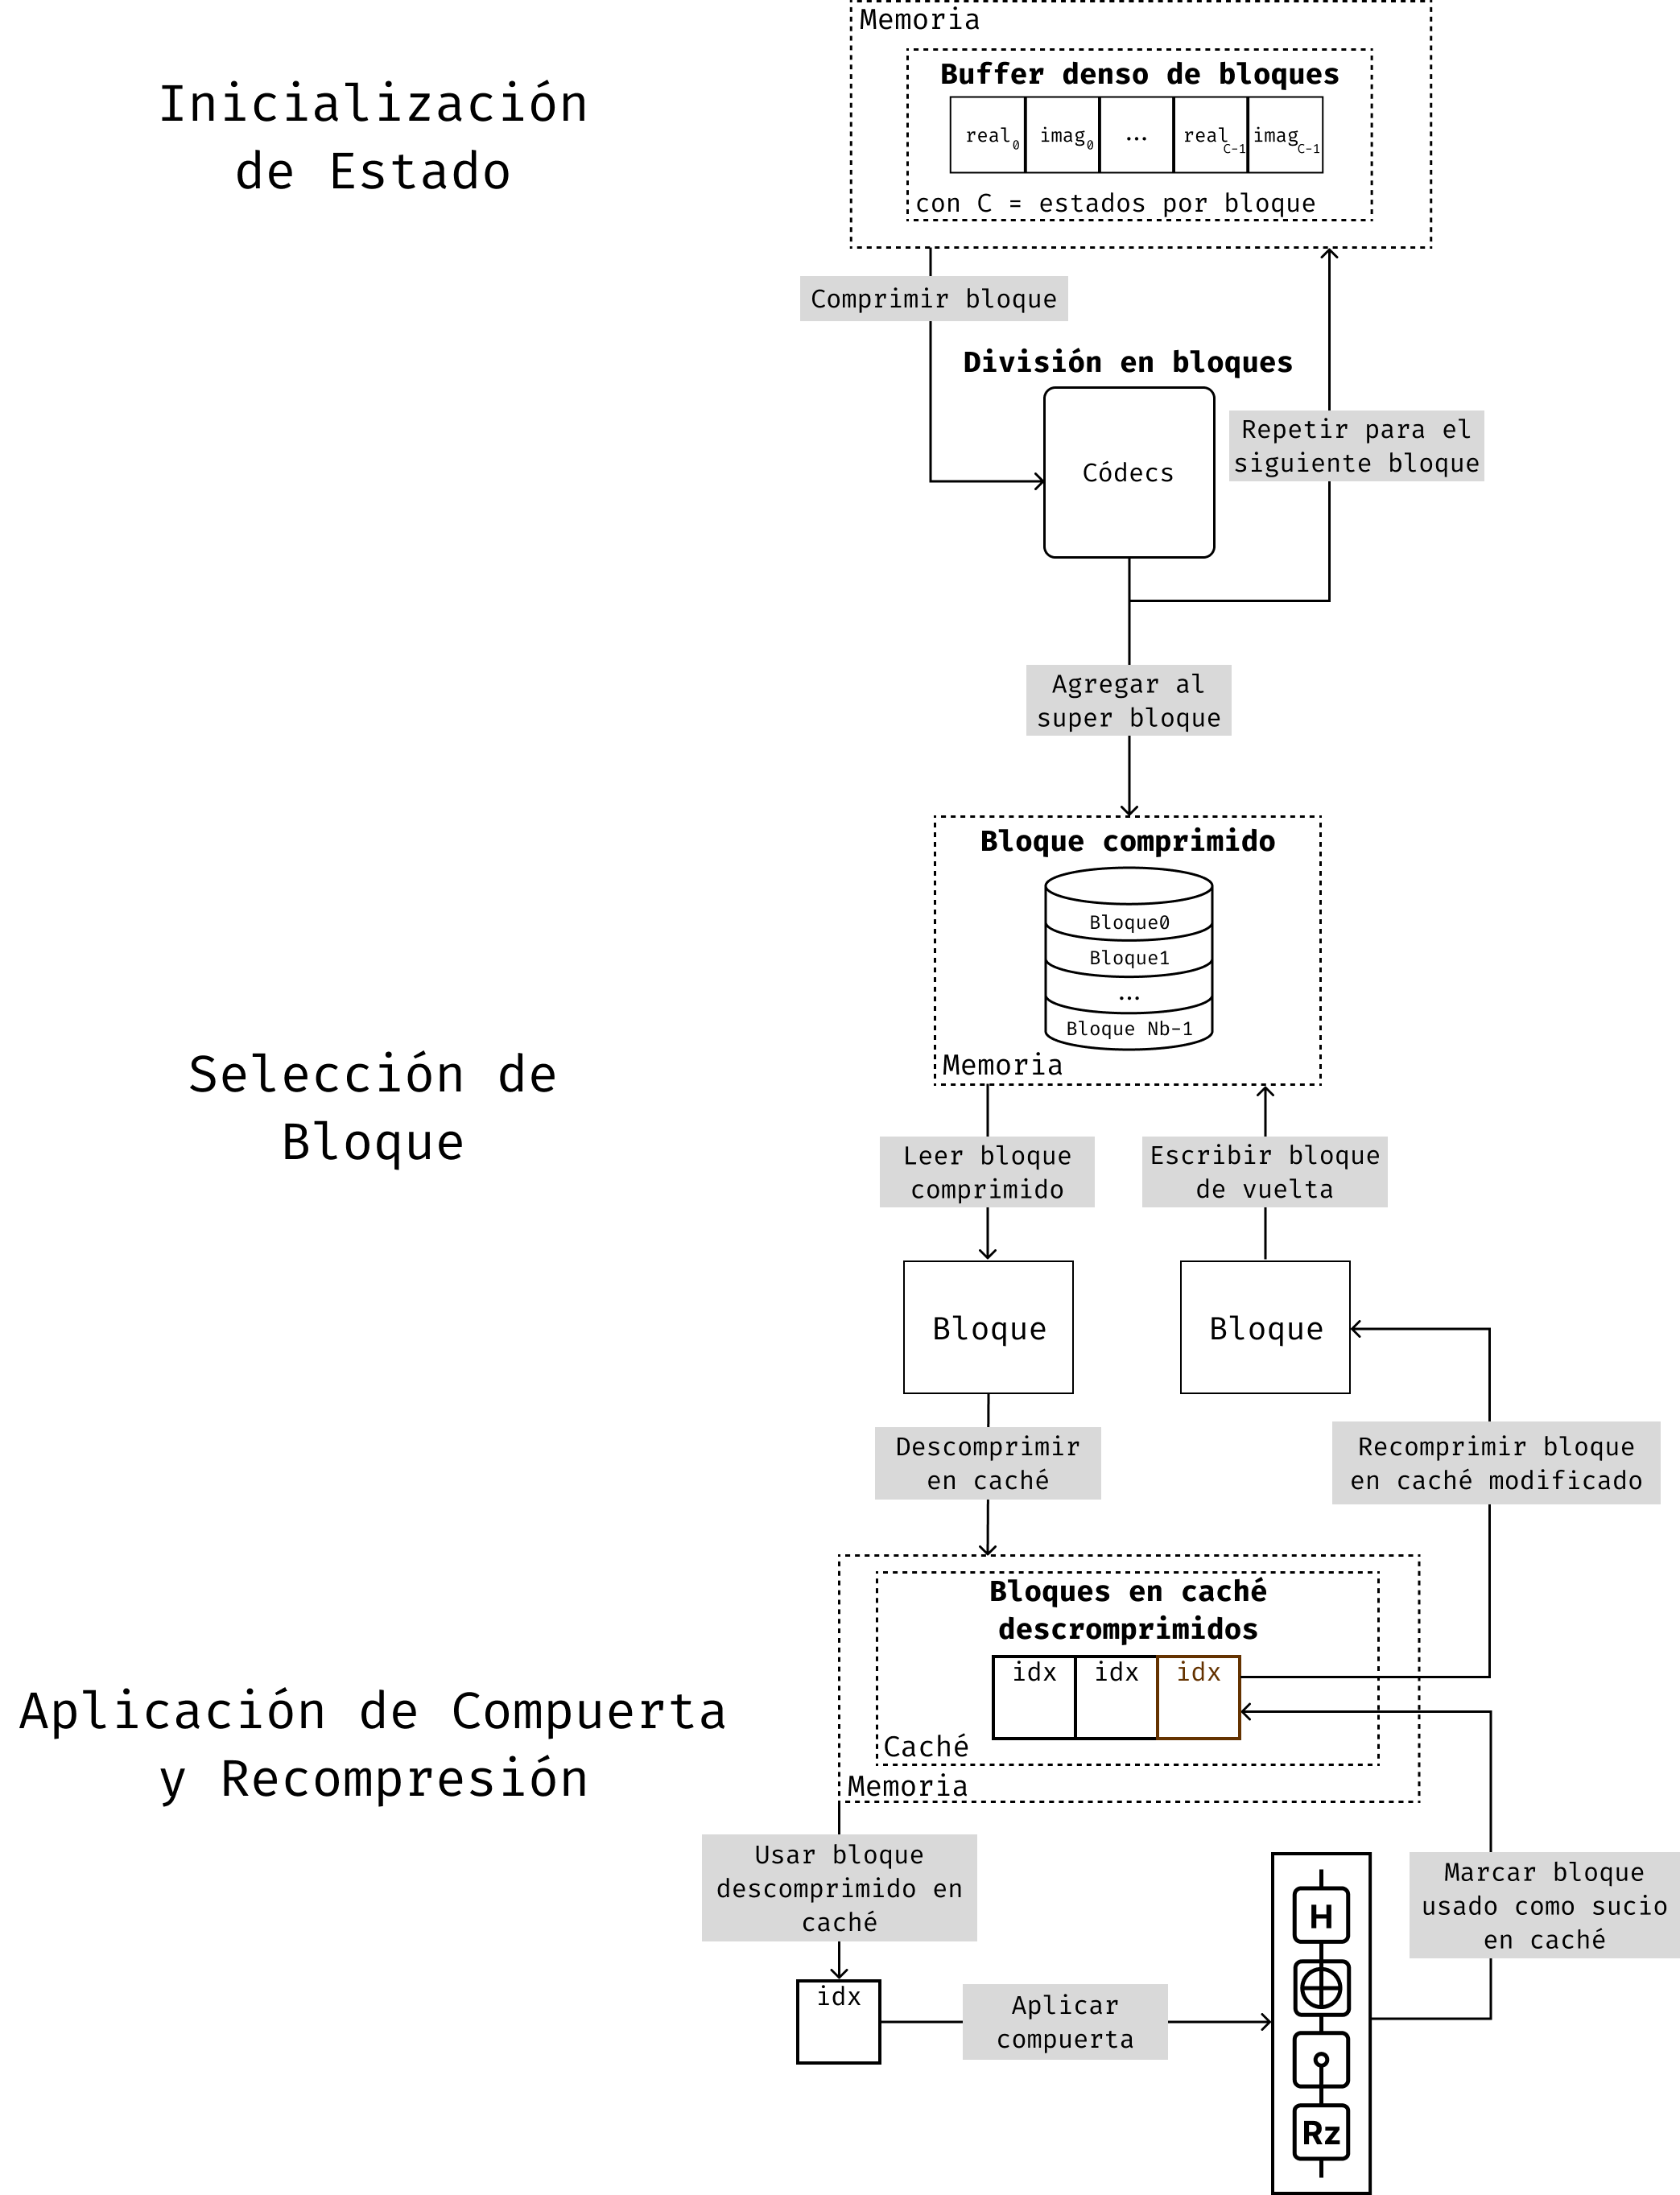
\includegraphics[height=1.15\textwidth]{images/development-architecture.png}
    \label{fig:simulation-design-architecture}
\end{figure}
